\section{Experimental Results} \label{sec:experimental}

\subsection{Values obtained in the laboratory} \label{subsec:experimental_measuredvalues}

Besides using Octave and Ngspice, it was possible to assemble the circuit shown in Figure \ref{fig:CircuitDraw} in a breadboard, for 5 different sets values for the resistances. The values of $C_1$, $C_2$, $R_3$ and $R_4$ remained constant, but the values of the remaining resistances were changed.
\par
Both in the lab and in the Ngspice simulations, the Texas Instruments $\mu A741$ OP-AMP model was used. In order to measure the input and output voltages, a signal generator was connected to the breadboard. The two channels of an oscilloscope were also connected to the breadboard. In these channels, respectively, the input and output voltage signals could be seen and both amplitudes were obtained. The oscilloscope's screen for Congiguration $\#$4 is shown in Figure \ref{fig:oscilloscope}; for the other configurations, similar signals were observed, but with different amplitudes. In Figure \ref{fig:breadboard}, the circuit assembled in the breadboard is shown.

\begin{figure}[H]
  \begin{subfigure}{.49\linewidth}
    \centering
    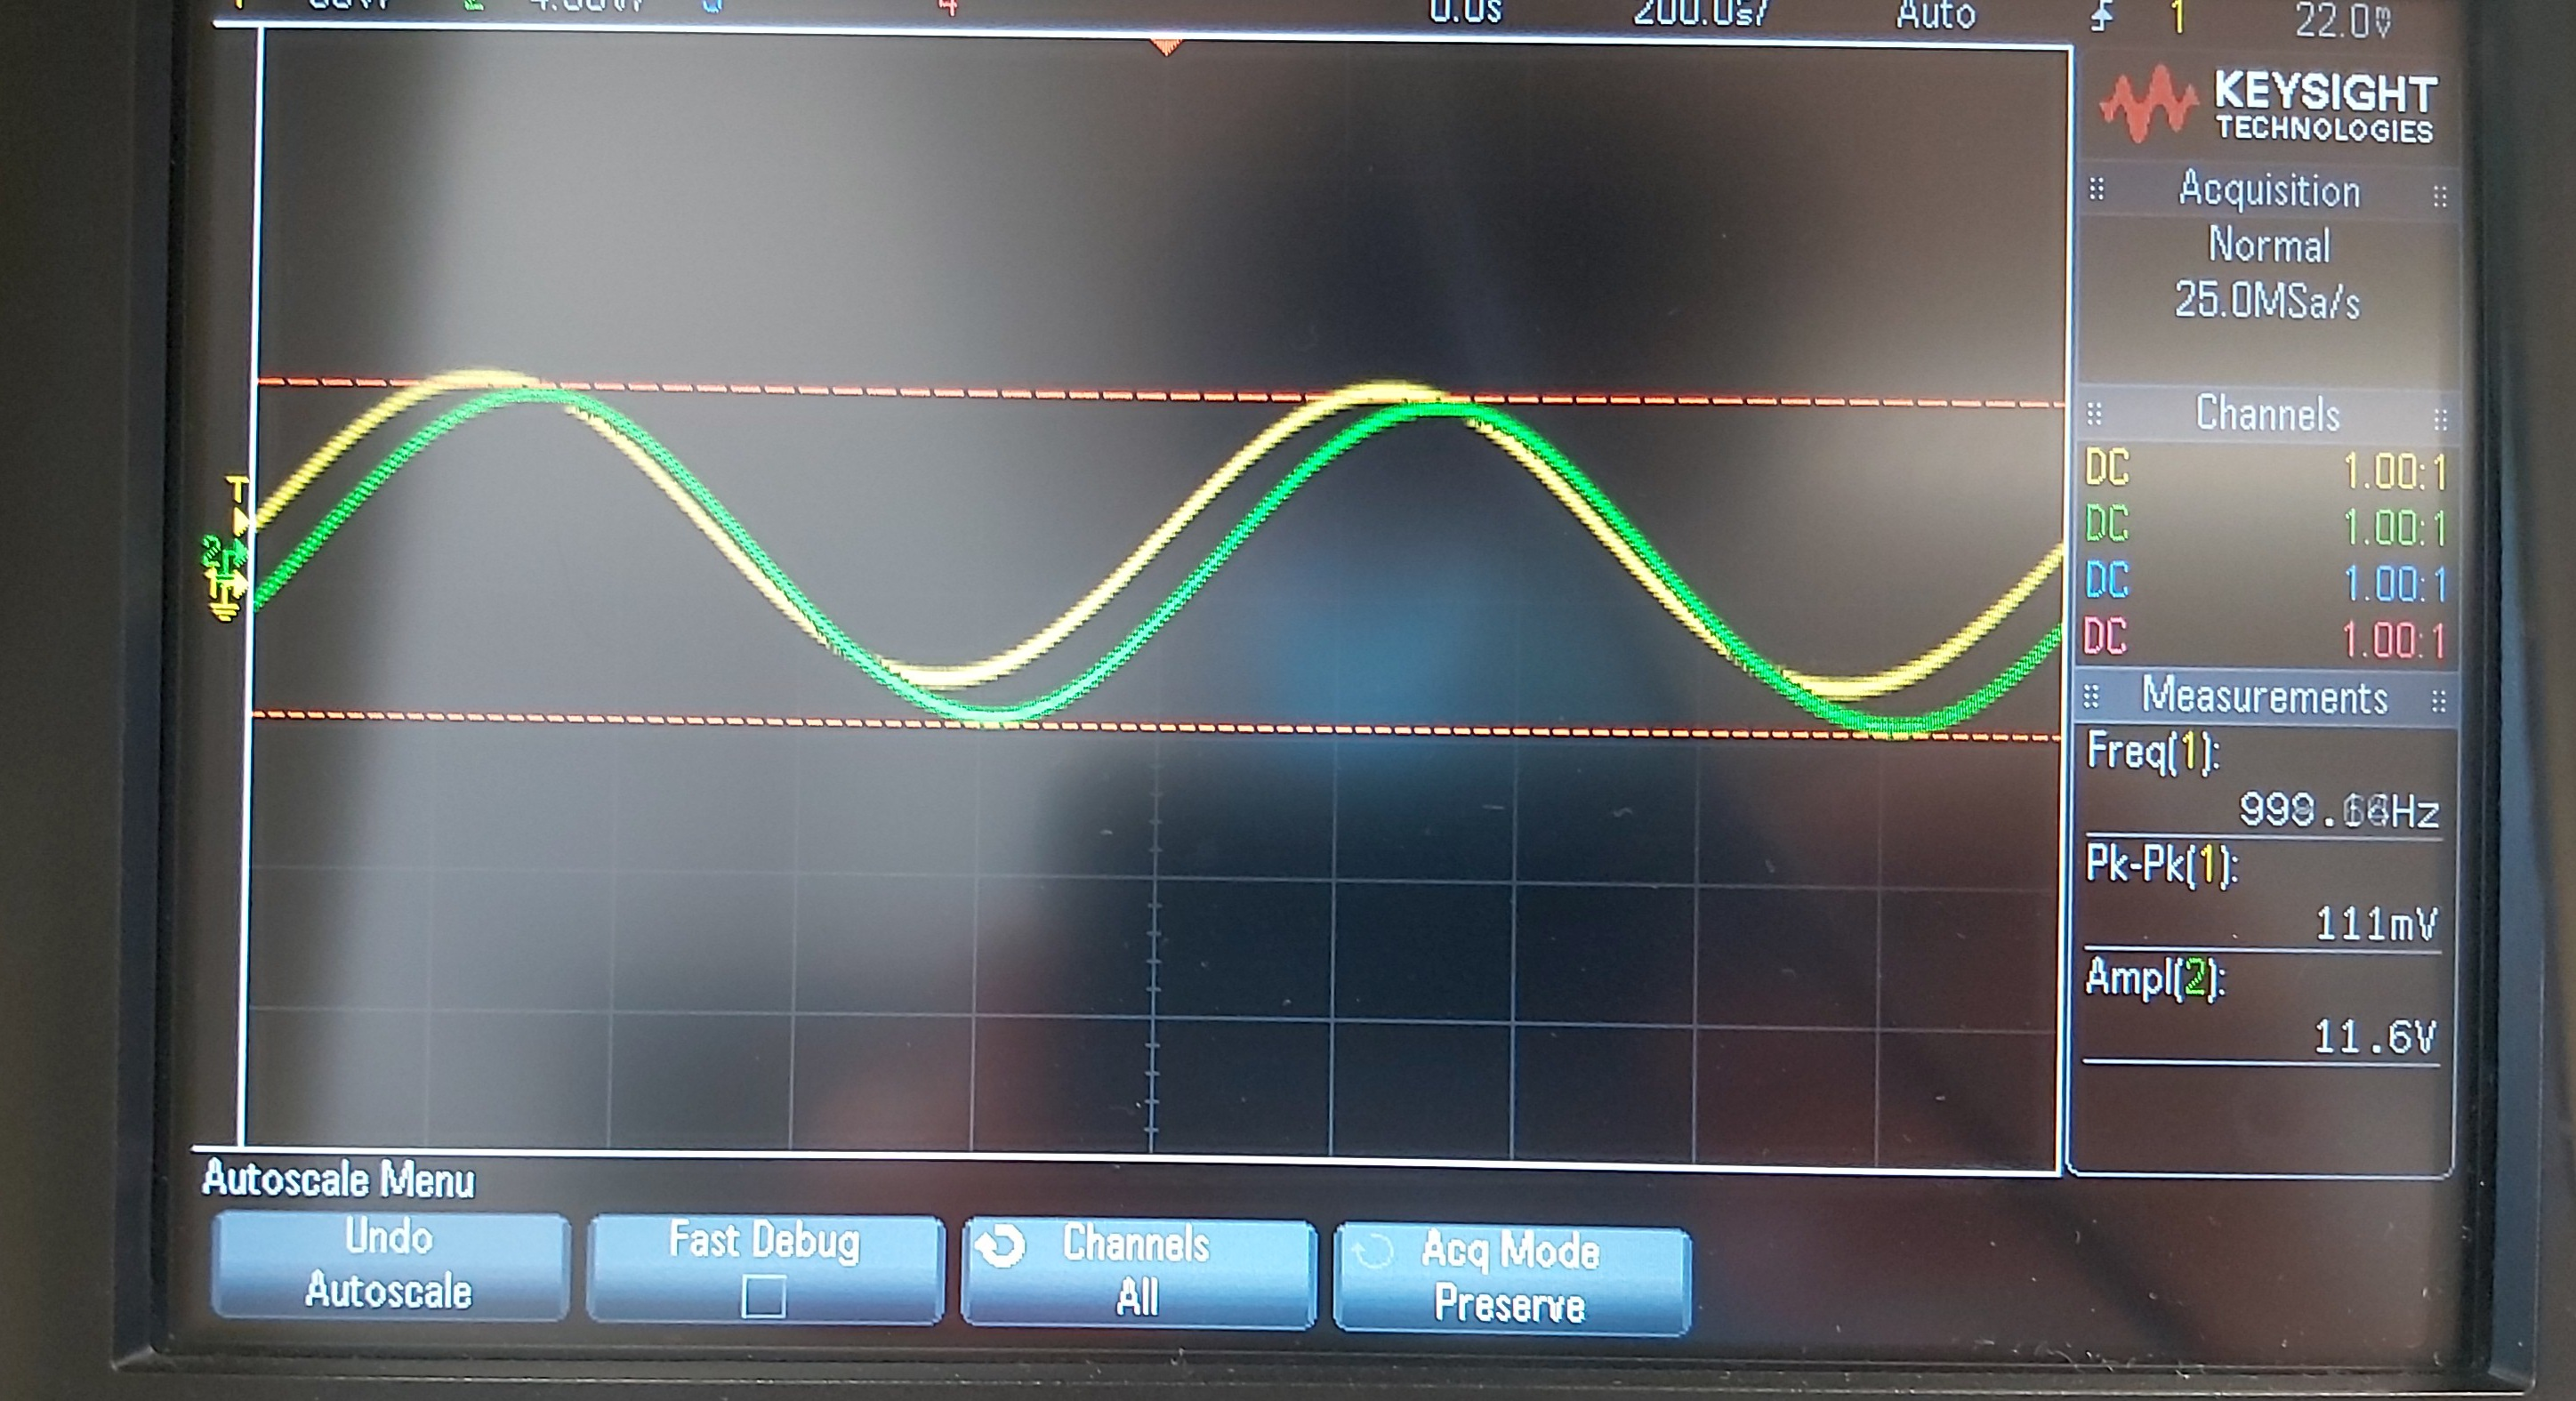
\includegraphics[width=0.95\linewidth]{../Oscilloscope4.jpeg}
    \footnotesize
  \caption{Input and output signals observed in the oscilloscope for configuration $\#$4 of resistances and capacitances' values}
   \label{fig:oscilloscope}
  \end{subfigure}
  \hspace{5mm}
  \begin{subfigure}{.49\linewidth}
    \centering
  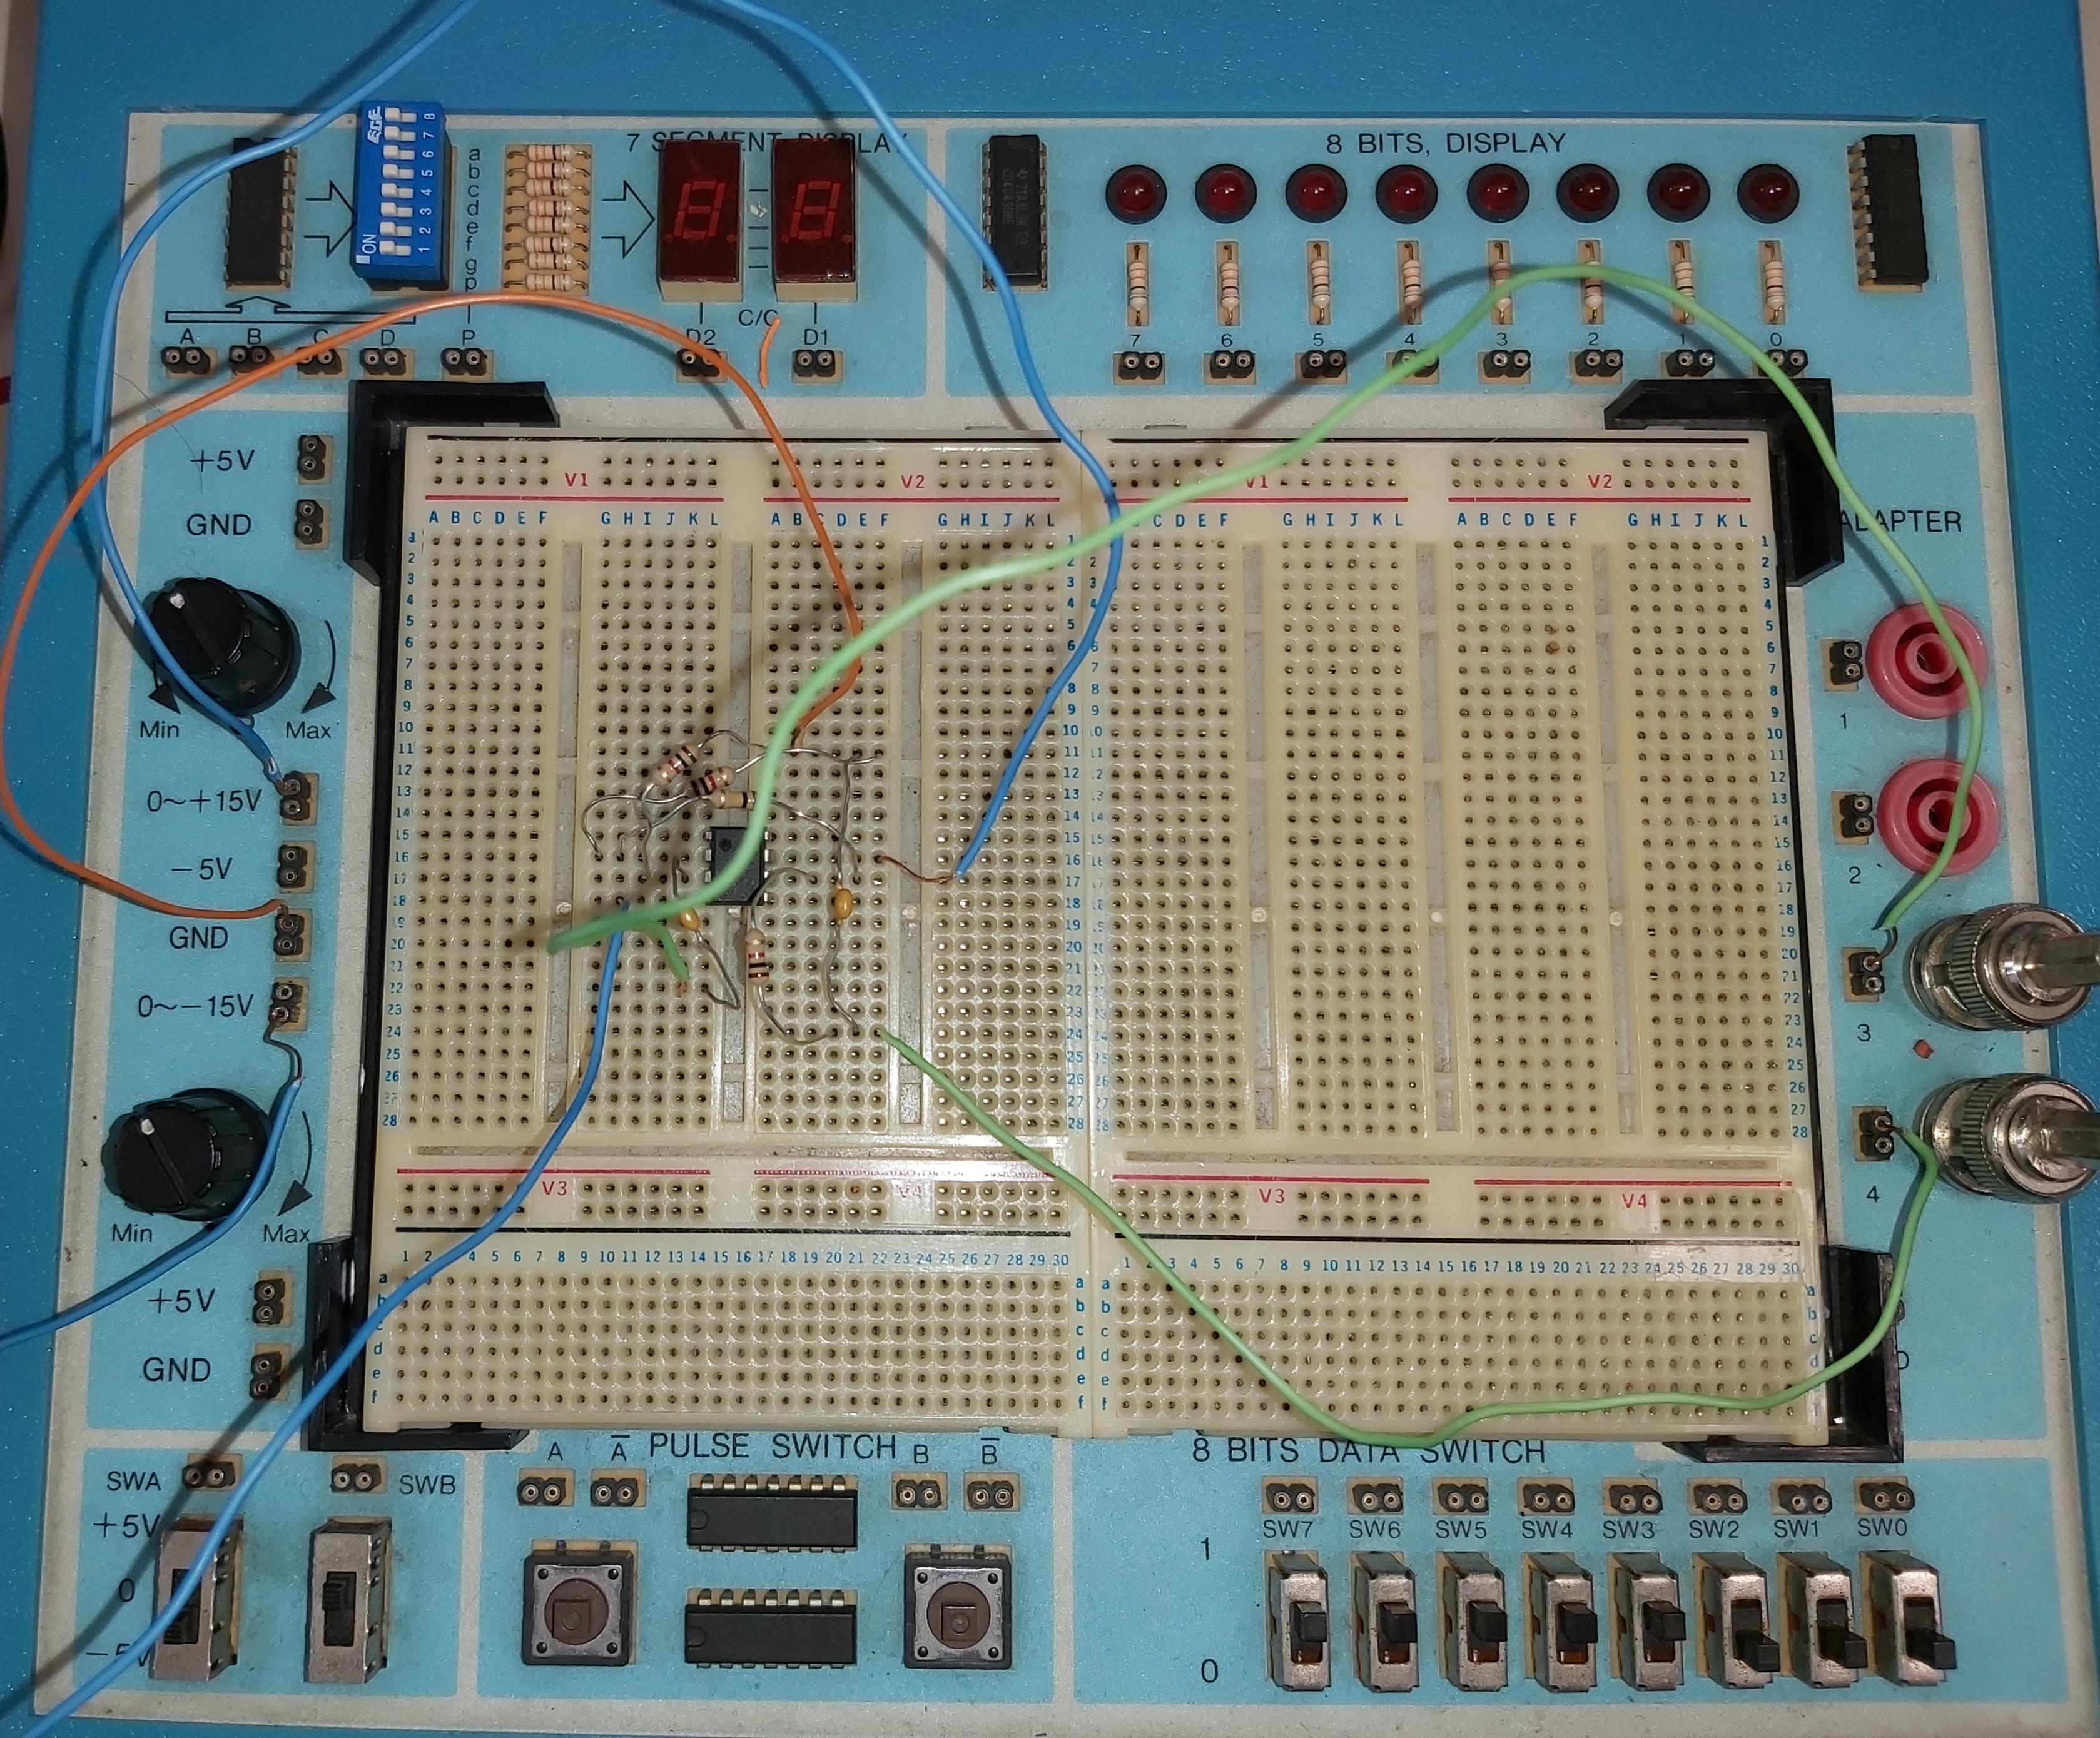
\includegraphics[width=0.95\linewidth]{../Breadboard.jpg}
  \caption{Circuit implemented in the breadboard during the laboratory class}
  \label{fig:breadboard}
  \end{subfigure}
\end{figure}

In Table \ref{tab:lab_results}, the results obtained for the five tested configurations are shown. A resistance of value $\infty$ indicates that that particular resistor wasn't used in the respective configuration. Even though the signal selected in the signal generator wasn't changed throughout the procedure, the frequency and the amplitudes measured in the oscilloscope varied slightly during each measurement, thus the values in the $Amp_{v_I}$ column below aren't the same. The gain in the last column is given by $Gain=\frac{Amp_{v_O}}{Amp_{v_I}}$.

\begin{table}[H]
    \centering
    \begin{tabular}{|c|c|c|c|c|c|c|c|}
        \hline
        Configuration $\#$ & $R_1$ & $R_2$ & $R_{2p}$ & $R_{4p}$ & $Amp_{v_I}$ [mV] & $Amp_{v_O}$ [V] & Gain [dB]\\
        \hline
        1 & 1 & 1 & $\infty$ & $\infty$ & 115 & 5.5 & 33.7 \\
        2 & 1 & 100 & $\infty$ & $\infty$ & 115 & 6.9 & 35.6 \\
        3 & 1 & 1 & $\infty$ & 1 & 113 & 9.5 & 38.5 \\
        4 & 1 & 1 & 2 & 1 & 111 & 11.6 & 40.4 \\
        5 & 1 & 1 & 1 & 1 & 113 & 13.0 & 41.2 \\
        \hline
    \end{tabular}
    \caption{Values obtained presencially in the laboratory; the resistances are in $k\;\Omega$. The gains are approximate values with one decimal point. The following values remained constant: $C_1=220\;nF$, $C_2=220\;nF$, $R_3=100\;k\Omega$ and $R_4=1\;k\Omega$.}
    \label{tab:lab_results}
\end{table}

\subsection{Simulation with the experimental values}

As seen in Table \ref{tab:lab_results}, configuration $\#$4 provided the gain most close to 4 dB. Thus, this configuration was also simulated in Ngspice, by using the same procedure which will be discussed in Section \ref{sec:simulation}. The input and output signals are plotted in Figure \ref{fig:out1_exp} and the gain in Figure \ref{fig:out2_exp}. The input and output signals were represented in order to notice the discrepancies between them and the signals seen in the oscilloscope, in Figure \ref{fig:oscilloscope}: the first as a slight visible difference from a sine or cosine wave function. However, in the oscilloscope, no visible ``distortion'' is clear. This may let us to believe that, even though the Ngspice model is very complex, it can't take into account all of the effects and phenomena that happen in an actual assembled circuit. As for the gain's plot, it's possible to verify that the frequency response clearly shows that the assembled circuit works as a bandpass filter, with the gain being maximum around a central frequency. As for the phase, the plot is very similar to the one that was obtained and will be analysed in Section \ref{sec:simulation}.

\begin{figure}[H]
  \begin{subfigure}{.49\linewidth}
    \centering
    \includegraphics[width=0.95\linewidth,trim=0mm 18mm 0mm 70mm,clip]{../sim/vo1_exp.pdf}
    \footnotesize
    \caption{Output signal variance with time for f=1kHz}
    \label{fig:out1_exp}
  \end{subfigure}
 % \hspace{5mm}
  \begin{subfigure}{.49\linewidth}
    \centering
    \includegraphics[width=0.95\linewidth,,trim=0mm 18mm 0mm 70mm,clip]{../sim/gain_exp.pdf}
    \caption{Gain}
    \label{fig:out2_exp}
  \end{subfigure}
  \centering
  \begin{subfigure}{.49\linewidth}
    \centering
    \includegraphics[width=0.95\linewidth,,trim=0mm 18mm 0mm 70mm,clip]{../sim/image_phase_exp.pdf}
    \caption{Phase}
    \label{fig:out3_exp}
  \end{subfigure}
\end{figure}

Finally, the same values computed for the theoretical analysis have been computed for the experimental results of configuration $\#$4 and by using Ngspice. These results are shown in Table \ref{tab:rip_exp}. The obtained gain is different from the gain calculated experimentally and shown in Table \ref{tab:lab_results}. Moreover, the central frequency is a bit off from the desired value, $f=1$ kHz. These observations once again show that the simulated Ngspice model does not represent the assembled circuit in a totally accurate way and that some effects are difficult or unable to be simulated. These results will be further analysed in Section \ref{sec:simulation} and compared to those obtained in the next Ngspice simulation.

\begin{table}[H]
  \centering
  \begin{tabular}{|c|c|}
    \hline    
        {\bf Designation} & {\bf Value [$\Omega$, Hz or dB]} \\ \hline
        \input{../sim/impedances_exp.tex}
        \input{../sim/valsim_exp_tab.tex}
  \end{tabular}
  \caption{Values obtained for the lower and higher cutoff frequencies (in Hz) and the final gain (in dB), for both the simulation and the theoretical analysis; bandwidth (in Hz) for the simulation.}
  \label{tab:rip_exp}
\end{table}
